\section{DiD Framework}


\begin{frame}{Group-Time Average Treatment Effects}

The \textbf{group-time average treatment effect}, $ATT(g,t)$, is a causal parameter in the context of DiD with multiple periods and multiple groups. The $ATT(g,t)$ has been approximated with the following estimators ($\tau$): \\
\vspace{5pt}
\begin{itemize}
    \item Outcome-regressions (Rubin, 1979) \\
    \vspace{3pt}
    $\tau^{reg} = N^{-1} \sum_{i=1}^{N}\{\hat{\mu_{1}}(X_{i}) - \hat{\mu_{0}}(X_{i}) \}$
    \vspace{-7pt}
    \item Inverse Probability Weighting (Rosenbaum, 1987) \\
    \vspace{3pt}
    $\tau^{ipw} = \frac{\sum_{i=1}^{N} Z_i Y_i / \hat{e}(X_i)}{\sum_{i=1}^{N} Z_i / \hat{e}(X_i)} - \frac{\sum_{i=1}^{N} (1-Z_i) Y_i / \{1 - \hat{e}(X_i)\}}{\sum_{i=1}^{N} (1-Z_i) / \{1 - \hat{e}(X_i)\}}$ \\
    \vspace{3pt}
    \footnotesize{where $\hat{e}$ is the estimated propensity score.} 
    \vspace{-7pt}
    \item Doubly-Robust Methods \\
    \vspace{3pt}
    $\tau^{dr} = \tau^{reg} + N^{-1} \sum_{i=1}^{N} \{ \frac{Z_i R_i}{\hat{e}(X_i)} - \frac{(1-Z_i) R_i}{1 - \hat{e}(X_i)} \}$ \\
    \vspace{3pt}
    \footnotesize{where $R_i = Y_i - \mu_{Z_{i}}(X_i)$ denotes the residual from outcome modeling.}
\end{itemize}
\end{frame}

\begin{frame}{A new estimator}
... blah blah blah ...
\end{frame}

\begin{frame}{Defining the g in ATT(g,t)}
Frequently, units are clustered before inference. For example, the ATT(g,t) may be evaluated on the zip code level. However, this can bias the estimation of a treatment effect because:
\vspace{5pt}

\begin{enumerate}
    \item Pre-defined borders may not be applicable in treatment context
    \item Biases of policymakers may be imposed on the study ex ante
\end{enumerate}
\vspace{5pt}

We can overcome this issue by \textbf{inferring the clusters ex post}, i.e. after obtaining individual-level treatment effects. Formally, we ...
\vspace{5pt}

\begin{enumerate}
    \item Measure idiosyncratic treatment effects over space and time, acknowledging that there will be missing treatment effects. 
    \item Interpolate missing treatment effects using the discrete subset we did measure.
    \item Divide the continuous set of treatment effects into k distinct clusters which represent approximations of the ATT(g,t) that are robust to spatial heterogeneity.  
\end{enumerate} 
\end{frame}

\begin{frame}{Defining the g in ATT(g,t): A Visualization}
The existence of zip codes can be attributed to a variety of historical, political, and administrative factors, but these divisions do not necessarily correspond to a population that is homogeneous in their treatment response.
\vspace{5pt}

  \begin{columns}
    % Split 1
    \begin{column}{0.4\linewidth}
    \centering
      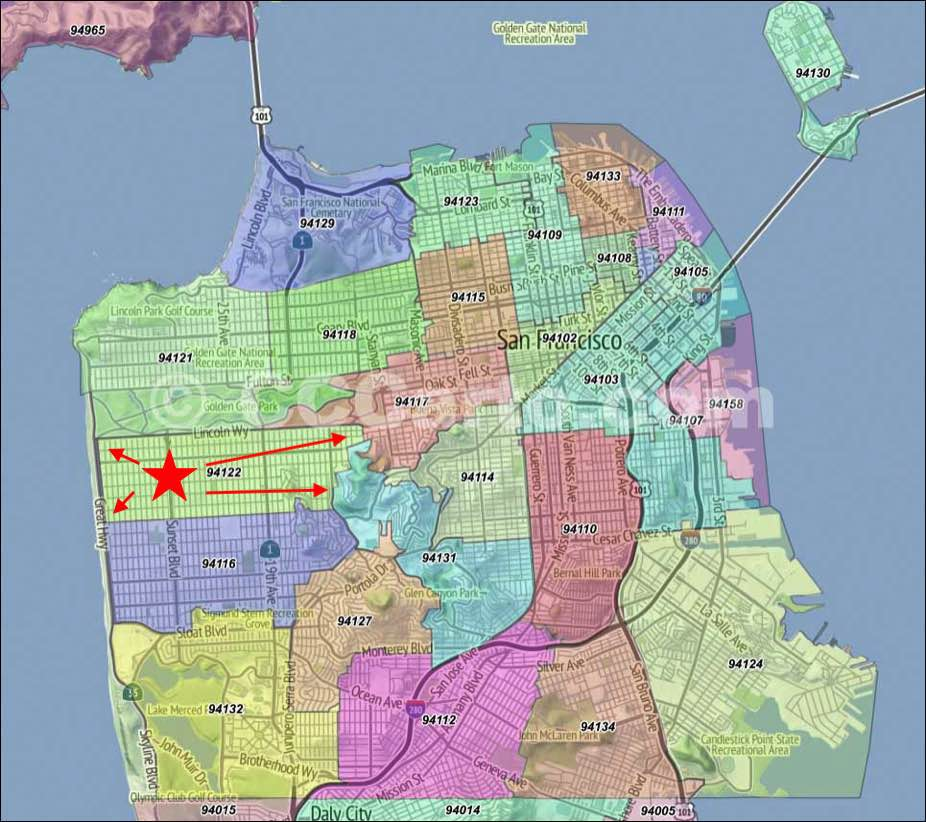
\includegraphics[scale=0.16]{figures/sf_zipcodes_exante.jpeg}
      \caption{\footnotesize{Ex Ante Comparison: Apples to Oranges}}
    \end{column}
    % Split 2
    \begin{column}{0.1\linewidth}
    \centering
      \Rightarrow
    \end{column}
    % Split 3
    \begin{column}{0.4\linewidth}
    \centering
      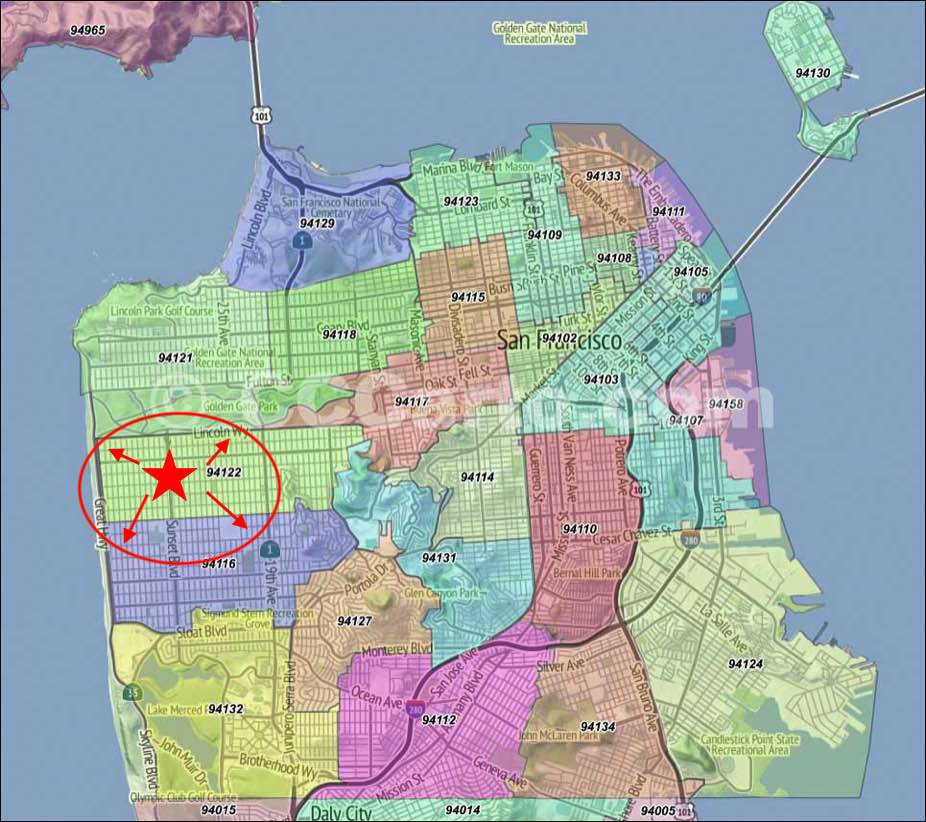
\includegraphics[scale=0.16]{figures/sf_zipcodes_expost.jpeg}
      \caption{\footnotesize{Ex Post Comparison: Apples to Apples}}
    \end{column}
  \end{columns}
\end{frame}

\begin{frame}{Control Strategy}
    Overlaying distributions of controls. This should also inform the clusters.
    More specifically: What if I can build the clusters based on all the covariates I consider and then represent them in a lower dimension in space???
\end{frame}

\begin{frame}{Limitations}
\begin{itemize}
    \item Vulnerable to structural differences in treatment effect density. Assumes the measurement of treatment effects across space and time distributed at random. 
\end{itemize}
    
\end{frame}